\chapter{Introduction}
\label{chap:intro}
Good feedback practices by tutors in one-on-one sessions are essential for self-regulated learning. For designing a good feedback practice, one needs to consider many factors. One of many principles to think about design and evaluation of self-created feedback procedures, is that feedback can be provided by a teacher, peer or tutor \parencite{nicol2006formative}. There is a discussion about what a good feedback strategy would inspire e.g. “facilitates the development of self-assessment” and “provides information to teachers that can be used to help shape teaching”. \\
Feedback comes in various forms and modes \parencite{narciss2008feedback} i.e. immediate vs. delayed feedback timing, single-try vs multiple-try, adaptive vs non-adaptive and implicit vs explicit feedback. In human-human-interactions, experienced tutors tend to provide indirect feedback to bring the attention of students to an error rather than giving corrective explicit feedback \parencite{lepper1990self}. Expert tutors also employ subtle techniques like delaying affirmation or expressing short hesitation when student inquires if he is doing alright, thus, hinting him about a mistake in the current step \parencite{fox1991cognitive}. There are other strategies like asking a leading question or subtly suggesting the student to redirect. On the other hand, it is argued that providing only implicit feedback can be detrimental. If a student spends too much time guessing for a solution or redirecting himself, it would be difficult for him to trace the path he took to solution \parencite{lewis1985discrimination}. Therefore, the tutoring strategy should be a trade-off between implicit and explicit feedback to allow room for the student to explore and learn from his mistakes, yet not be confused or stuck at an impasse.\\
The argument has frequently been made that one way to achieve the effectiveness of human tutoring in educational contexts is by using intelligent tutoring systems, embodied agents and robots \cite{intro1}. A recent survey of long-term human-robot interaction (HRI) highlighted the increasing popularity of using social robots in educational environments \cite{survey1}. Studies recording attitude of children towards robot show positive outcomes \cite{oh2010social}. Although, there are a lot of unexplored topics in this field. While prior research has attempted and succeeded to develop emotionally intelligent and personalized robot tutors, most of these employ explicit feedback methods such as informing the student that answer is wrong, or some step is wrong or giving hints on how to solve the problem \parencite{gordon2016affective}\parencite{ramachandran2019personalized}. To the best of our knowledge, no robot tutoring system has been used to study the effectiveness of implicit strategies to provide feedback to students in one-on-one tutoring sessions. Moreover, there is not enough discussion on spatial reasoning skills \parencite{yilmaz2017development} in robot tutoring while it has been established that such skills augment geometric and mathematical understanding of students \parencite{keren2012kindergarten}. Most of the studies are limited to teaching languages \parencite{gordon2016affective} and solving mathematical problems \parencite{ramachandran2019personalized}. \\
\begin{figure}[h]
   \centering
%   \includegraphics[width=\textwidth,height=\textheight,keepaspectratio]{fig_3-4}
   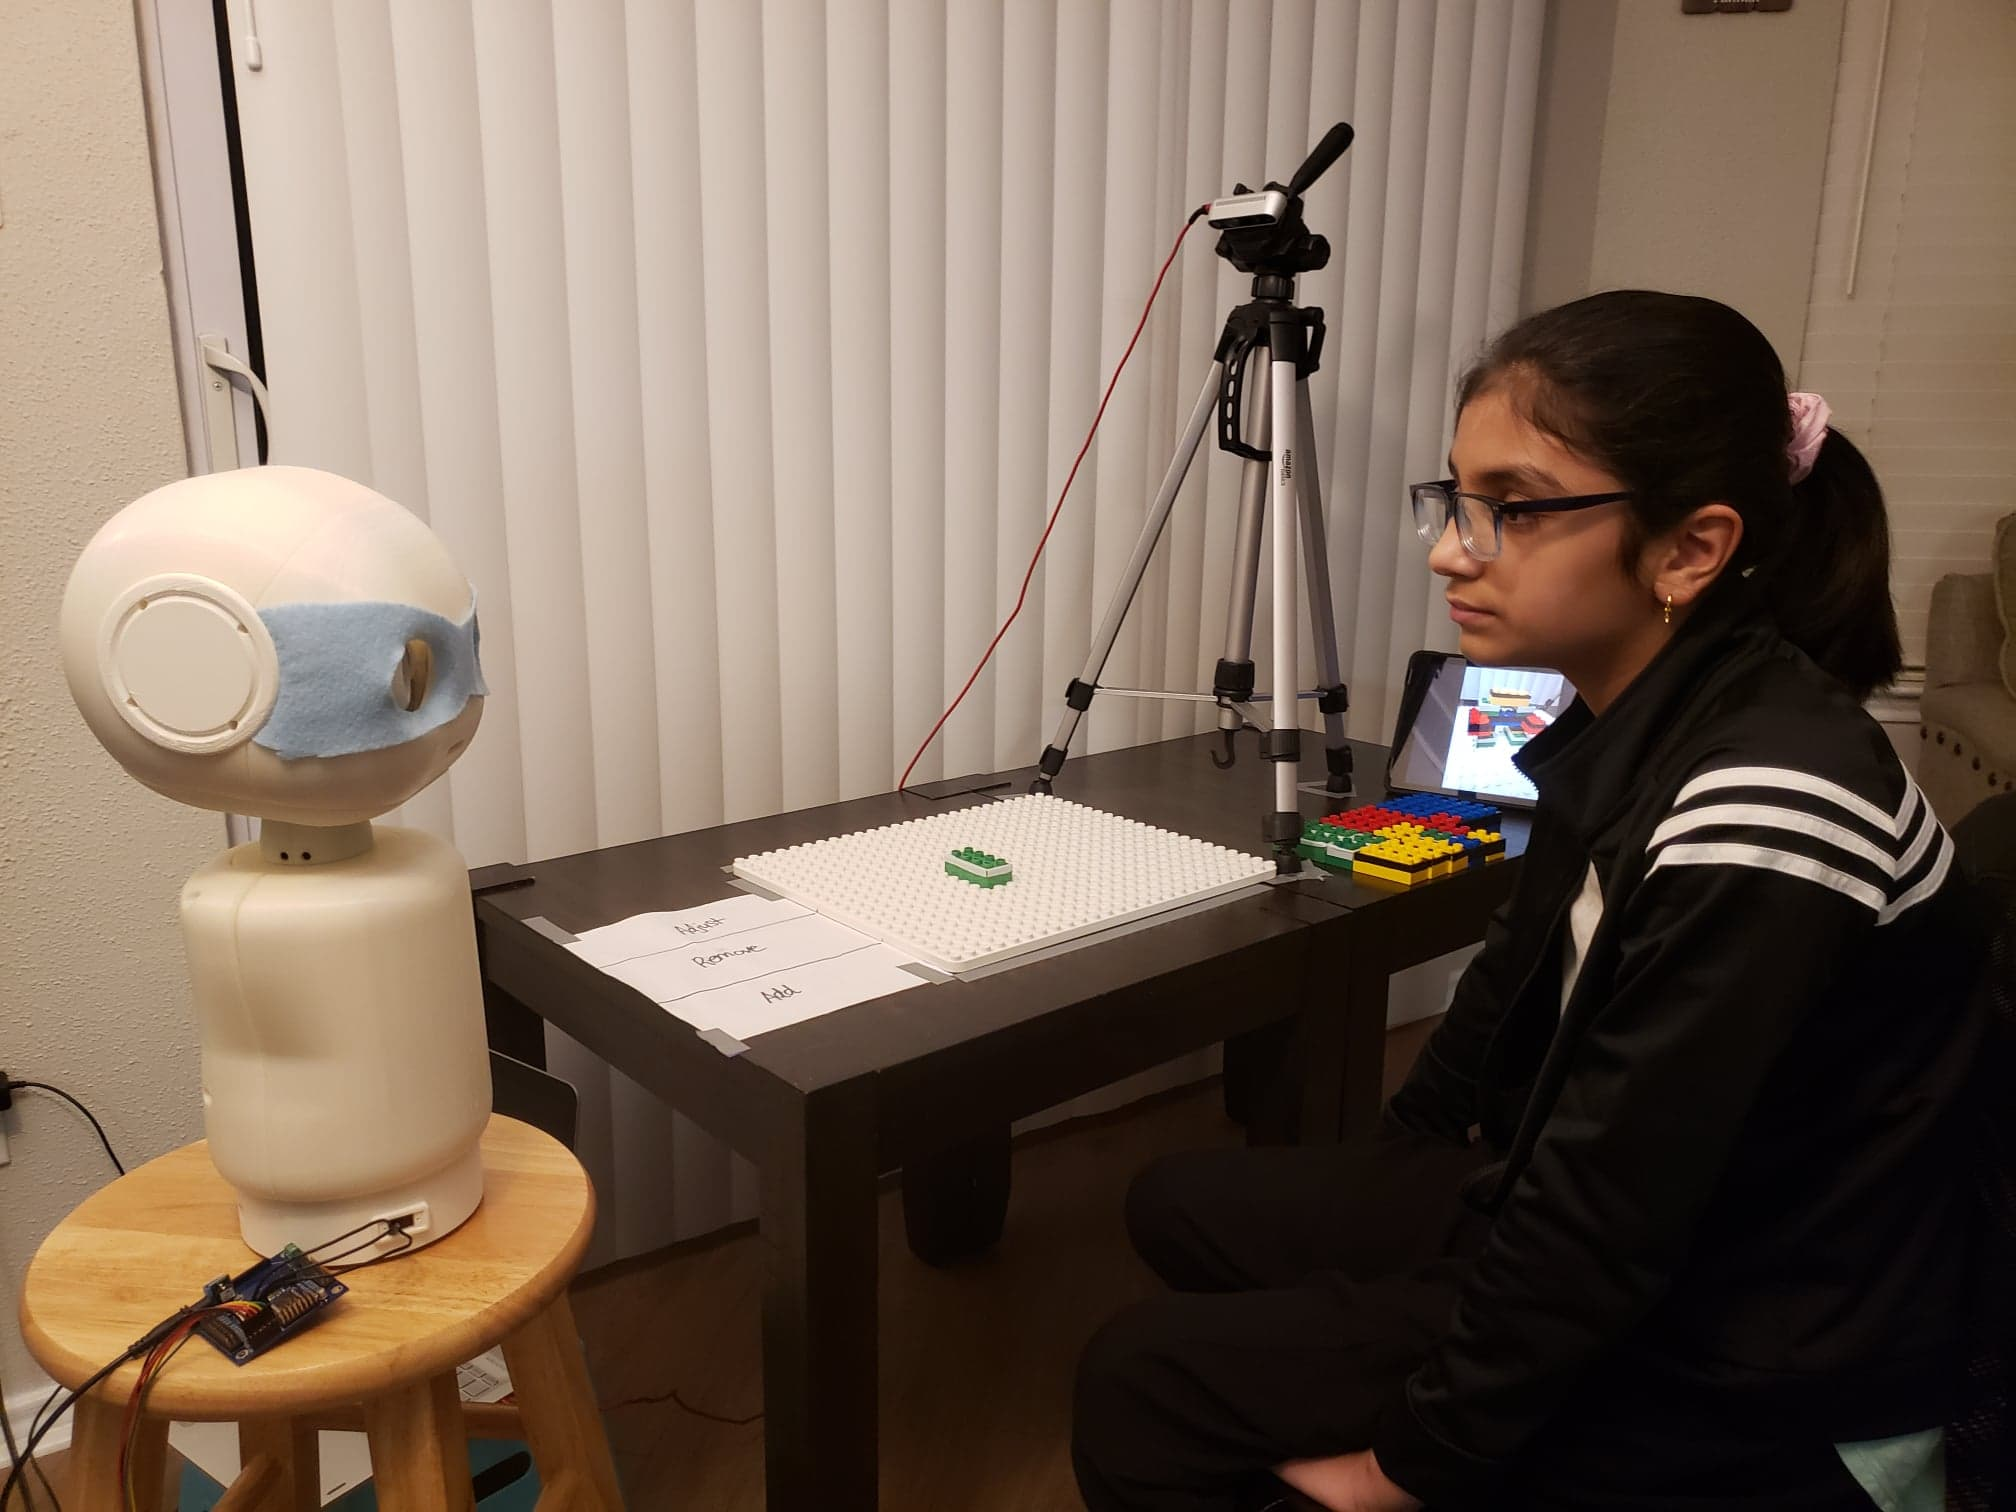
\includegraphics[width = 1\textwidth,trim={2cm 0 4cm 5cm},clip]{figures/s1.jpg}
   \caption[{System Setup}]{System Setup}
   \label{fig:fig_1-1}
\end{figure}
We contextualized our investigation into a one-on-one tutoring session. The set up is shown in figure \ref{fig:fig_1-1}.  The setup consists of the following:
\begin{enumerate}
    \item Perception system: To track actions of the participant. 
    \item Intelligent Robot Tutor: Acts as a tutor to provide feedback based on actions of the participant.
    \item 3D blocks: Serves as the playground for the participant to solve designed spatial reasoning task. 
\end{enumerate}
We collected data from our participant to evaluate the impact of implicit and explicit feedback on self-efficacy and learning gain, and her perception of such robot tutor while working on a spatial reasoning task. Analysis of data has resulted in useful design implications for our detailed study. We believe that this study opens an interesting research space in robot tutoring. Future studies about tradeoff between implicit and explicit feedback, effectiveness of various types of implicit feedback, its personalization and right timing for intervention etc. will follow. Resulting design implications will advance research in this rather unexplored direction. \\
In the next chapter, we review prior work in field of social robotics for education, feedback practices in tutoring, and development, importance and augmentation of spatial reasoning in early ages. We give background to our study. This review is followed by a description of our system and how the exploratory study is designed along with evaluation. We then discuss our findings and their implications for future work, concluding with a summary of our contributions.

